\documentclass[journal]{IEEEtai}

\usepackage[colorlinks,urlcolor=blue,linkcolor=blue,citecolor=blue]{hyperref}

\usepackage{color,array}

\usepackage{graphicx}

\usepackage{soul}

\usepackage{makecell}
\usepackage{graphicx}
\usepackage{textcomp}
\usepackage{array} 
\usepackage{longtable}
\usepackage{booktabs}
\usepackage{float}
\usepackage{subcaption}
\usepackage{amsmath}
%% \jvol{XX}
%% \jnum{XX}
%% \paper{1234567}
%% \pubyear{2020}
%% \publisheddate{xxxx 00, 0000}
%% \currentdate{xxxx 00, 0000}
%% \doiinfo{TQE.2020.Doi Number}

\newtheorem{theorem}{Theorem}
\newtheorem{lemma}{Lemma}
\setcounter{page}{1}
%% \setcounter{secnumdepth}{0}


\begin{document}


\title{INT104 CW2-Lab report} 


\author{Ruiyang.Wu\quad	sID:2257475\quad E-Mail:Ruiyang.Wu22@student.xjtlu.edu.cn
	\\
	TA: Yu Kang \quad E-Mail:yu.kang23@student.xjtlu.edu.cn
}

\markboth{INT104 Artificial Intelligence CW2 2024/05/09 Ruiyang.Wu}
{INT104 Artificial Intelligence CW2 2024/05/09 Ruiyang.Wu}

\maketitle



\section{\textbf{Introduction}}

\IEEEPARstart{I}{n} this experiment, I first separated `Programme'=3 to convert the task of this experiment from a four-classification problem into a three-classification. Then, the remaining students were classified in `Programme' using Support Vector Machine (SVM), decision tree, Random Forest, Naïve Bayes and Integrated Classifiers as required by the task. In each classification method, I performed a grid search for the combination of input features with the choice of hyperparameters, while evaluating the performance using cross-validation to select the optimal case while ensuring that it does not lead to over-fitting. In addition, due to the category imbalance, this experiment also attempts to improve the performance of classification for samples with `Programme'=2 using under-sampling and Synthetic Minority Over-sampling Technique (SMOTE). Finally, conjectures about the selection of hyperparameters and feature combinations with relation to classification performance are presented. To ensure the reproducibility of the experiment, relevant results and code are saved in the following repository: 
\href{https://github.com/MushihimePepsi/XJTLU_ICS_Y2S2_Course-notes_23-24/tree/main}{\ul{https://github.com/MushihimePepsi/XJTLU\_ICS\_Y2S2\\\_Course-notes\_23-24/tree/main}}


\section{\textbf{Declarations on feature selection, prevention of over-fitting and class-imbalance}}
\subsection{\textbf{Feature selection}}
Although the PCA method was used in CW1 to perform dimensionality reduction by selecting directions (linear combinations of the original features) that explain as much variance as possible in the dataset, with the expectation that the selection of these new features would serve as better classifier inputs. In practice, however, this behavior does not lead to better classification performance, so in this report, the inputs to the classifiers will all be combinations of the original features.

Similarly, although the importance of features can be ranked using Random Forest or the most important features can be selected using Recursive Feature Elimination (RFE), the optimal feature inputs tend to be different for different classifiers in actual training, so in this experiment each classifier is trained using the most suitable set of features. A Grid search study of the best input features for different classifiers has been placed in the \href{https://github.com/MushihimePepsi/XJTLU_ICS_Y2S2_Course-notes_23-24/tree/main/INT104-%E4%BA%BA%E5%B7%A5%E6%99%BA%E8%83%BD}{\ul{repository}} as a reference for you.
\\\\\\
\begin{figure}[htbp]
	\centerline{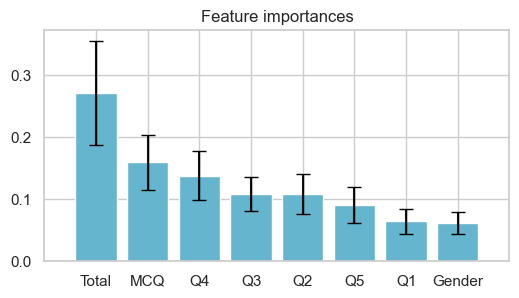
\includegraphics[width=18pc]{Feature importances.png}}
	\caption{Random Forest Estimation of Feature Importance}
\end{figure}

\subsection{\textbf{Prevention of over-fitting}}
In this experiment, due to the small size of the dataset, it is necessary to pay special attention to prevent over-fitting of the model. The k-fold cross validation method was used in the process of training the model by setting k=5, dividing the training set into 5 parts, and using 4 parts for model training and 1 part for validation each time, preventing the model from only relying on a single training set and enhancing the generalization ability. In addition, regularization or adding a penalty term to the loss function to limit the complexity of the model is also performed on the hyperparameters setting of the classifier. Finally, the test and training sets were divided in a ratio of 3:7 to test as many diverse samples as possible while ensuring sufficient training samples.

\subsection{\textbf{Mitigating class-imbalance}}
The distribution of classes in the dataset of this experiment is not balanced, excluding the very small proportion of `Programme'=3 samples, the number of `Programme'=2 samples is about half of the number of `Programme'=1 or `Programme'=4 samples, leading to the problem of class imbalance, where some of the classifiers, although they perform better overall (Accuracy $\approx$ 0.7), are were unable to effectively categorize the samples with `Programme'=2. To solve this problem, under-sampling and SMOTE operations are adopted in this experiment to reduce the model's over-dependence on the categories with more samples and improve the generalization ability.


\section{\textbf{Separation of samples with `Programme'=3}}
In CW1, I demonstrated that due to the high correlation of `Programme'=3 students with `Grade'=3 features, this relationship can be utilized to pre-separate `Programme'=3 students, so that the feature dimensionality and the complexity of classifying other subsequent Programmes can be reduced.
\begin{table}[htbp]  
	\caption{Predicting 'Programme'=3 with feature 'Grade'=3} % 添加表格标题 
	\centering % 将表格居中显示  
	\begin{tabular}{|c|c|c|}  
		\hline  
		\textit{Confusion Matrix} & \textbf{True Programme=3} & \textbf{True Programme$\neq$3} \\ \hline  
		\textbf{Pred. Programme=3} & TP=35 & FP=3 \\ \hline  
		\textbf{Pred. Programme$\neq$3} & FN=0 & TN=581 \\ \hline  
	\end{tabular}   
\end{table}

\renewcommand\arraystretch{1.3}%保证每列高度是原先的1.5倍
\begin{table}[htbp]%星号表示双栏
	\caption{Performance of the classification by 'Grade'}
	\begin{tabular}{p{1.7cm}<{\centering}p{1.7cm}<{\centering}p{1.7cm}<{\centering}p{1.7cm}<{\centering}p{1.7cm}<{\centering}}%设定每列的宽度以及对齐方式,并且可以做到自动换行
		\Xhline{1.2pt}%第一条粗线
		\textbf{Precision} & \textbf{Recall} & \textbf{Accuracy} & \textbf{F1 Score}  \\ 
		\Xhline{1.2pt}%第二条粗线
		92.1\% & 100\% & 99.5\% & 95.9\% \\ 
		\Xhline{1.2pt}%第三条粗线
	\end{tabular}
	\label{MRFsum}
\end{table}

This categorization performed quite well, and subsequent operations in this paper will focus on separating the remaining samples for `Programme'=\{1,2,4\}. Since there are 38 students (6.14\%) with `Programme'=3, the total sample size is reduced from 619 to 581 after this step of processing, and the feature `Grade' is also removed.

\section{\textbf{Task1: Decision tree \& Random forest}}
After comparison, this experiment uses Gini impurity rather than information gain as a measure of the importance level of features and constructs decision trees using the CART algorithm. The decision tree is regularized and pruned and the best parameters are selected by a restricted grid search for 'max\underline{ }depth', 'min\underline{ }samples\underline{ }split' and 'min\underline{ }samples\underline{ }split'. It ensures that the decision tree has good classification performance while having proper generalization ability.

\renewcommand\arraystretch{1.2}%保证每列高度是原先的1.5倍
\begin{table}[htbp]%星号表示双栏
	\caption{Performance of several typical input feature combinations}
	\begin{tabular}{p{2.5cm}<{\centering}p{1.3cm}<{\centering}p{1.5cm}<{\centering}p{1.7cm}<{\centering}p{0.8cm}<{\centering}}%设定每列的宽度以及对齐方式,并且可以做到自动换行
		\Xhline{1.2pt}%第一条粗线
		\textbf{Features} & \textbf{max\underline{ }depth} & \textbf{Accuracy} & \textbf{`Programme'=2 F1-Score}  \\ 
		\Xhline{1.2pt}%第二条粗线
		'MCQ', 'Q1', 'Q4' & 4 & 61.7\% & 0\% \\ 
		\Xhline{1.2pt}%第二条粗线
		'Gender', 'MCQ', 'Q3', 'Q4' & 6 & 61.1\% & 40\% \\ 
		\Xhline{1.2pt}%第二条粗线
		'MCQ', 'Q1', 'Q2' & 8 & 60.0\% & 24\% \\ 
		\Xhline{1.2pt}%第三条粗线
		'Gender', 'Total', 'MCQ', 'Q1', 'Q2', 'Q3', 'Q4', 'Q5' & 6 & 54.9\% & 17\% \\ 
		\Xhline{1.2pt}%第三条粗线
	\end{tabular}
	\label{MRFsum}
\end{table}
It can be observed that different input features have a significant impact on classification and do not conform to previous predictions of importance. The deeper the tree, the more overfitting it tends to be, and the better the classification performance for `Program'=2. Taking into account performance, select `MCQ', `Q1', `Q3', and `Q4' as input features.
\begin{figure}[htbp]
	\centerline{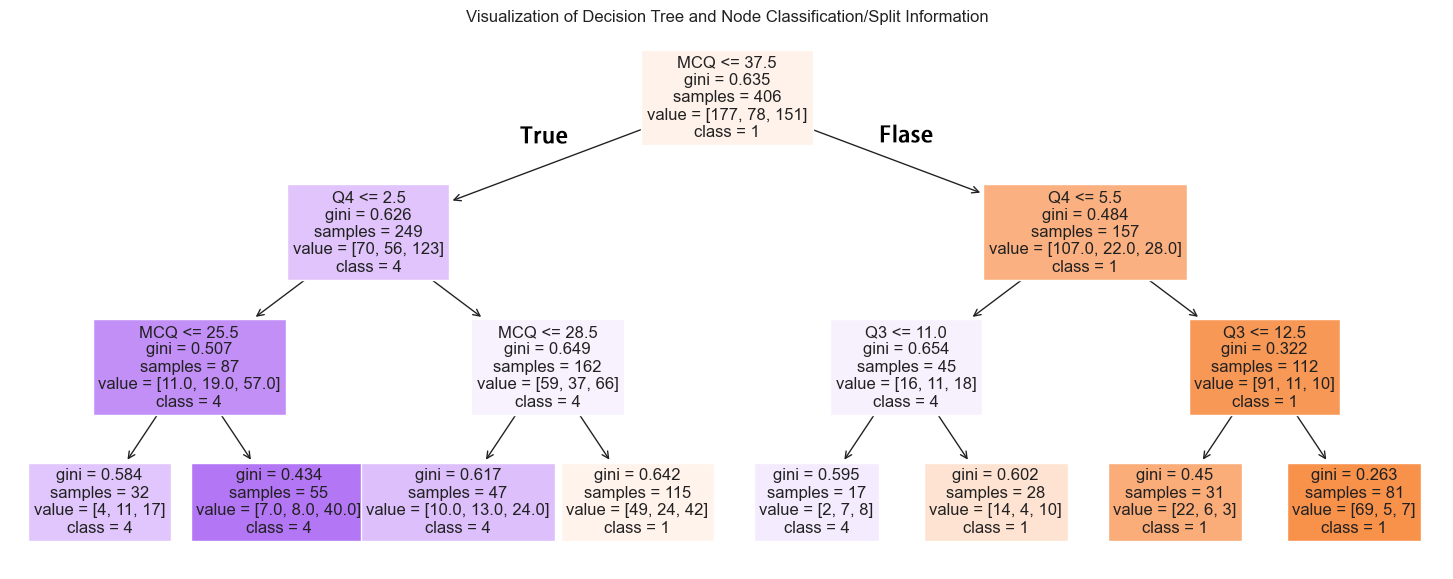
\includegraphics[width=18.2pc]{Visualization of Decision Tree+TF.png}}
	\caption{Visualization of Decision Tree and Node Classification/Split Information}
\end{figure}

\renewcommand\arraystretch{1.3}%保证每列高度是原先的1.5倍
\begin{table}[htbp]%星号表示双栏
	\caption{Weighted performance of Decision Tree}
	\begin{tabular}{p{1.7cm}<{\centering}p{1.7cm}<{\centering}p{1.7cm}<{\centering}p{1.7cm}<{\centering}p{1.7cm}<{\centering}}%设定每列的宽度以及对齐方式,并且可以做到自动换行
		\Xhline{1.2pt}%第一条粗线
		\textbf{Accuracy} & \textbf{Recall} & \textbf{Precision} & \textbf{F1 Score}  \\ 
		\Xhline{1.2pt}%第二条粗线
		60.5\% & 60.6\% & 46.9\% & 52.8\% \\ 
		\Xhline{1.2pt}%第三条粗线
	\end{tabular}
	\label{MRFsum}
\end{table}

Random forests combine the practices of bagging and random subspace method while randomly sampling the samples and sample features of the training set. Such an approach enhances the differences and independence between base learners, resulting in an integrated model with less variance, better generalization and natural resistance to over-fitting. It can be seen that despite the similarity of Accuracy, Random Forest enhances the Precision of prediction.
\renewcommand\arraystretch{1.3}%保证每列高度是原先的1.5倍
\begin{table}[htbp]%星号表示双栏
	\caption{Weighted performance of Random forests}
	\begin{tabular}{p{1.7cm}<{\centering}p{1.7cm}<{\centering}p{1.7cm}<{\centering}p{1.7cm}<{\centering}p{1.7cm}<{\centering}}%设定每列的宽度以及对齐方式,并且可以做到自动换行
		\Xhline{1.2pt}%第一条粗线
		\textbf{Accuracy} & \textbf{Recall} & \textbf{Precision} & \textbf{F1 Score}  \\ 
		\Xhline{1.2pt}%第二条粗线
		61.1\% & 61.1\% & 60.3\% & 60.1\% \\ 
		\Xhline{1.2pt}%第三条粗线
	\end{tabular}
	\label{MRFsum}
\end{table}

	% 假设你已经有了两张图片文件  
	% 使用 subcaption 环境将两个 figure 环境放在一起  
\begin{figure}[htbp]  
	\begin{subfigure}[b]{0.24\textwidth} % 你可以调整这个值来改变图片的宽度  
		\centering  
		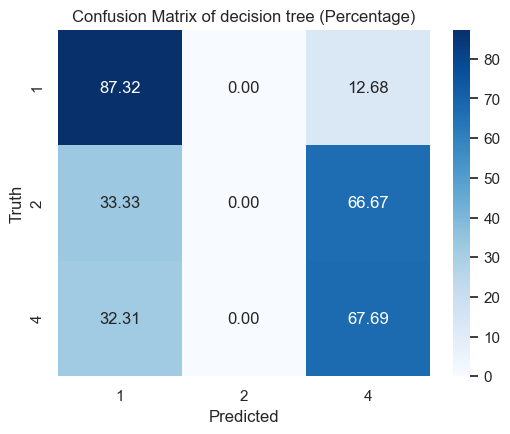
\includegraphics[width=\textwidth]{Confusion Matrix of decision tree.png}  
		\caption{Confusion Matrix of decision tree (Percentage)}  
	\end{subfigure}  
	\hfill % 这将在两个子图之间添加一些水平填充,但不会换行  
	\begin{subfigure}[b]{0.24\textwidth}  
		\centering  
		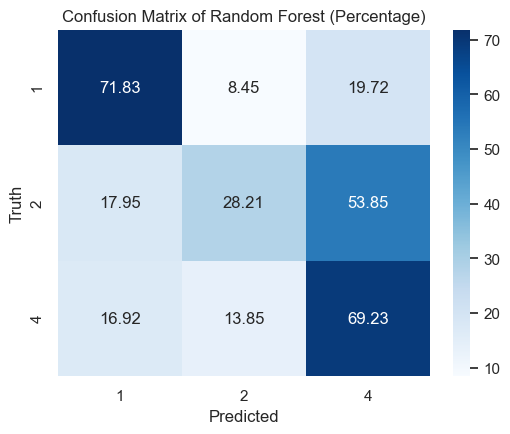
\includegraphics[width=\textwidth]{Confusion Matrix of Random Forest.png}  
		\caption{Confusion Matrix of Random Forest (Percentage)}  
	\end{subfigure}  
	\caption{Comparison of Classification Effectiveness of Decision Trees and Random Forests} % 总的标题  
\end{figure}

\section{\textbf{Task2: Support Vector Machine}}
Support Vector Machine (SVM) maps input data to high-dimensional feature spaces through kernel functions, making originally nonlinear separable data linearly separable in the feature space while avoiding dimensionality disasters. Using the multi classification strategy of OVR (One Versus Rest), different kernel functions are searched on the grid to adjust the degree of softness and hardness of the decision boundary, and the influence range of the kernel function, gamma, to find the most suitable parameter\{`C': 10, `gamma': `scale', `kernel': `rbf'\}. Due to class imbalance, the regularized training set is under-sampled as input to improve the classification performance of `Programme'=2.
\begin{table}[htbp]%星号表示双栏
	\caption{Weighted performance of SVM}
	\begin{tabular}{p{1.7cm}<{\centering}p{1.7cm}<{\centering}p{1.7cm}<{\centering}p{1.7cm}<{\centering}p{1.7cm}<{\centering}}%设定每列的宽度以及对齐方式,并且可以做到自动换行
		\Xhline{1.2pt}%第一条粗线
		\textbf{Accuracy} & \textbf{Recall} & \textbf{Precision} & \textbf{F1 Score}  \\ 
		\Xhline{1.2pt}%第二条粗线
		60.5\% & 60.5\% & 63.6\% & 61.5\% \\ 
		\Xhline{1.2pt}%第三条粗线
	\end{tabular}
	\label{MRFsum}
\end{table}

\begin{figure}[htbp]
	\centerline{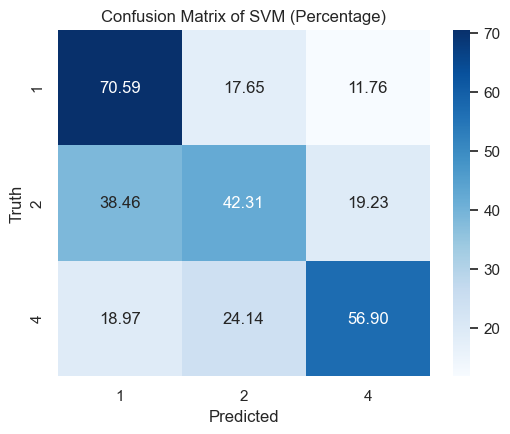
\includegraphics[width=14pc]{Confusion Matrix of SVM.png}}
	\caption{Confusion Matrix of SVM (Percentage)}
\end{figure}

\section{\textbf{Task3: Naïve Bayes}}
Naïve Bayes works based on Bayes' theorem and the assumption of conditional independence of features, by counting the a priori probability and conditional probability finally using Bayes' theorem to find out the posterior probability, and ultimately selecting the category with the largest a posteriori probability as the classification result. The input features are identified as 'Gender', 'Total', 'Q1', 'Q2', 'Q3', 'Q4', 'Q5' after grid search.

\begin{center}
\text{\textbf{Select largest posterior probability class as prediction}}
\begin{align} 
	P(B_k|A)&=\frac{P(A|B_  k) \cdot P(B_k)}{\sum_{1}^{n}P(B_i)P(A|B_i) }
	=\frac{P(A|B_k) \cdot P(B_k)}{P(A)}
	\\ 
	\hat{y}&=arg max_k P(C_k|x)
	\\
	h_{nb}(x)&=argmax_{c\in y}P(c)\prod_{i=1}^{d}P(x_i|c)
\end{align}
\text{Probability of A: P(A); Conditional probability: P(B$|$A)}
\end{center}

\begin{table}[htbp]%星号表示双栏
	\caption{Weighted performance of Gaussian Naïve Bayes}
	\begin{tabular}{p{1.7cm}<{\centering}p{1.7cm}<{\centering}p{1.7cm}<{\centering}p{1.7cm}<{\centering}p{1.7cm}<{\centering}}%设定每列的宽度以及对齐方式,并且可以做到自动换行
		\Xhline{1.2pt}%第一条粗线
		\textbf{Accuracy} & \textbf{Recall} & \textbf{Precision} & \textbf{F1 Score}  \\ 
		\Xhline{1.2pt}%第二条粗线
		63.6\% & 63.6\% & 62.9\% & 63.0\% \\ 
		\Xhline{1.2pt}%第三条粗线
	\end{tabular}
	\label{MRFsum}
\end{table}

\begin{figure}[htbp]
	\centerline{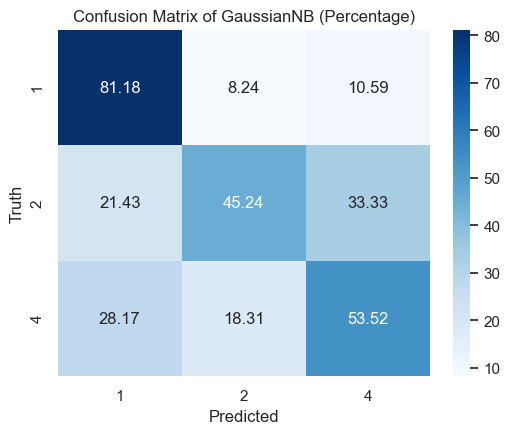
\includegraphics[width=14pc]{Confusion Matrix of GaussianNB.png}}
	\caption{Confusion Matrix of Gaussian Naïve Bayes (Percentage)}
\end{figure}

\section{\textbf{Task4: Ensemble classifier}}
In integrated learning, in addition to the previously used random forests and the unexplained adaBoost method, I used voting to combine previously trained models, expecting to produce a single strong classifier out of multiple weak classifiers. However voting produces models with mediocre performance. Furthermore, although soft voting is often thought to provide more accurate predictions, in practice it is weaker than hard voting. This may be due to the homogeneity of the base classifiers and incorrect weight selection.

\begin{table}[htbp]%星号表示双栏
	\caption{Weighted performance of Gaussian Naïve Bayes}
	\begin{tabular}{p{1.4cm}<{\centering}p{1.4cm}<{\centering}p{1.4cm}<{\centering}p{1.4cm}<{\centering}p{1.4cm}<{\centering}p{1.4cm}<{\centering}}%设定每列的宽度以及对齐方式,并且可以做到自动换行
		\Xhline{1.2pt}%第一条粗线
		\textbf{Vote type} & \textbf{Accuracy} & \textbf{Recall} & \textbf{Precision} & \textbf{F1 Score}  \\ 
		\Xhline{1.2pt}%第二条粗线
		Hard & 58.9\% & 58.9\% & 54.8\% & 54.1\% \\ 
		\Xhline{1.2pt}%第三条粗线
		Soft & 57.7\% & 57.7\% & 52.4\% & 53.8\% \\ 
		\Xhline{1.2pt}%第三条粗线
	\end{tabular}
	\label{MRFsum}
\end{table}

	% 假设你已经有了两张图片文件  
% 使用 subcaption 环境将两个 figure 环境放在一起  
\begin{figure}[htbp]  
	\begin{subfigure}[b]{0.24\textwidth} % 你可以调整这个值来改变图片的宽度  
		\centering  
		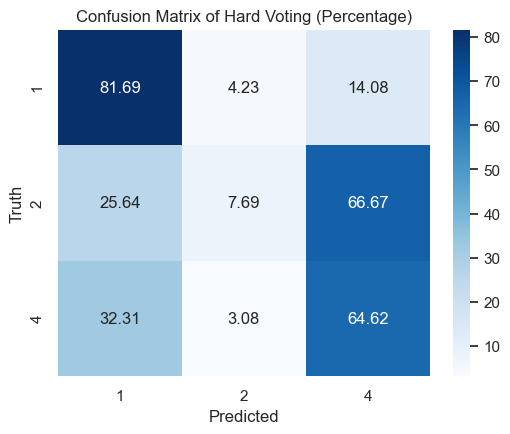
\includegraphics[width=\textwidth]{Confusion Matrix of Hard Voting.png}  
		\caption{Confusion Matrix of Hard Voting (Percentage)}  
	\end{subfigure}  
	\hfill % 这将在两个子图之间添加一些水平填充,但不会换行  
	\begin{subfigure}[b]{0.24\textwidth}  
		\centering  
		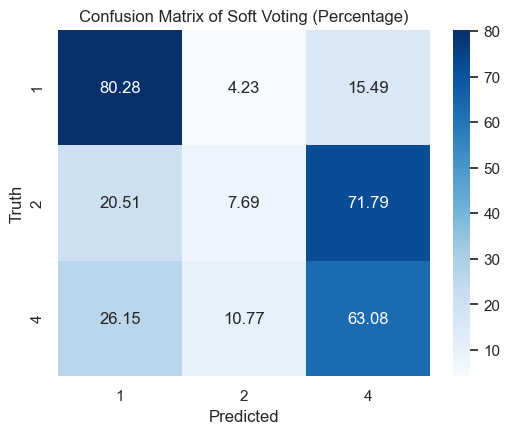
\includegraphics[width=\textwidth]{Confusion Matrix of Soft Voting.png}  
		\caption{Confusion Matrix of Soft Voting (Percentage)}  
	\end{subfigure}  
	\caption{Comparison of Classification Effectiveness of Hard Voting and Soft Voting} % 总的标题  
\end{figure}

\section{\textbf{Conclusions, limitations and conjectures}}
In this experiment, I performed a grid search under cross-validation for each class of classifiers, and also investigated different combinations of input features, making conjectures between feature combinations and classifier performance to find different combinations of features suitable for each classifier. 

This study, still, has the limitation of separating the `Programme'=3 at very beginning of the classification with a view to simplifying the subsequent classification process. But samples of `Programme'=3 themselves still contain information that is distinct from the other categories and may be useful in supervised learning to separate the other categories. In addition, the new feature set obtained after dimensionality reduction was not used in this experiment, and although PCA dimensionality reduction does not give much impact on the results, non-linear dimensionality reduction methods such as Locally Linear Embedding (LLE) can still be used to extract relational features of the data in higher dimensions to obtain better classification performance.

\section{\textbf{Acknowledgment}}
I would like to thank the two TAs of SC375: Yu Kang and Yiqiang Cai for their detailed comments and guidance, Dr. Shengchen Li for his careful design of the experiments.





\end{document}
